
\documentclass{article}

\setlength{\oddsidemargin}{0.05 in}
\setlength{\evensidemargin}{-0.05 in}
\setlength{\topmargin}{-0.6 in}
\setlength{\textwidth}{6.5 in}
\setlength{\textheight}{9.5 in}
\setlength{\headsep}{0.25 in}
\setlength{\parskip}{0.1 in}

%
% ADD PACKAGES here:
\usepackage [usenames] {color}
\definecolor {infocolor} {rgb} {0.6,0.6,0.6}
\definecolor {steel blue}{rgb}{0.274510,0.509804,0.705882}
\everymath{\color{steel blue}}
\everydisplay{\color{steel blue}}
%
\usepackage{tikz}
\usetikzlibrary{calc}

\usepackage{rotating}

\usepackage{amsmath,amsfonts,amssymb,enumerate,graphicx}

%
% The following commands set up the lecnum (lecture number)
% counter and make various numbering schemes work relative
% to the lecture number.
%
\newcounter{lecnum}
\renewcommand{\thepage}{\thelecnum-\arabic{page}}
\renewcommand{\thesection}{\thelecnum.\arabic{section}}
\renewcommand{\theequation}{\thelecnum.\arabic{equation}}
\renewcommand{\thefigure}{\thelecnum.\arabic{figure}}
\renewcommand{\thetable}{\thelecnum.\arabic{table}}

\DeclareMathOperator{\rk}{rk}

\newcommand{\tran}{^{\mbox{\tiny $\top$}}}
\newcommand{\tleq}{^{\mbox{\tiny $\leqslant$}}}
\newcommand{\teq}{^{\mbox{\tiny $=$}}}

%
% The following macro is used to generate the header.
%
\newcommand{\lecture}[2]{
   \pagestyle{myheadings}
   \thispagestyle{plain}
   \newpage
   \setcounter{lecnum}{#1}
   \setcounter{page}{1}
   \noindent
   \begin{center}
       \vbox{\vspace{2mm}
         \hbox {\leftline{\Large LECTURE #1: \hfill}}
         \vspace{3mm}
         \hbox {\leftline{\Large #2 \hfill}}
         \vspace{4mm}
         \hrule
         \vspace{3mm}
         \hbox to 6.5in { {{\Large \sc Combinatorial Optimization - Polyhedral Theory}  \hfill Mar. 2015} }
         \vspace{3mm}
        }
   \end{center}
   \markboth{LECTURE #1: #2}{LECTURE #1: #2}
   \pagenumbering{arabic}
   \vspace*{4mm}
}
%
% Convention for citations is authors' initials followed by the year.
% For example, to cite a paper by Leighton and Maggs you would type
% \cite{LM89}, and to cite a paper by Strassen you would type \cite{S69}.
% (To avoid bibliography problems, for now we redefine the \cite command.)
% Also commands that create a suitable format for the reference list.
\renewcommand{\cite}[1]{[#1]}
\def\beginrefs{\begin{list}%
        {[\arabic{equation}]}{\usecounter{equation}
         \setlength{\leftmargin}{2.0truecm}\setlength{\labelsep}{0.4truecm}%
         \setlength{\labelwidth}{1.6truecm}}}
\def\endrefs{\end{list}}
\def\bibentry#1{\item[\hbox{[#1]}]}

%Use this command for a figure; it puts a figure in wherever you want it.
%usage: \fig{NUMBER}{SPACE-IN-INCHES}{CAPTION}
\newcommand{\fig}[3]{
            \vspace{#2}
            \begin{center}
			Figure \thelecnum.#1:~#3
			\end{center}
	}
% Use these for theorems, lemmas, proofs, etc.
\newtheorem{theorem}{Theorem}[lecnum]
\newtheorem{lemma}[theorem]{Lemma}
\newtheorem{proposition}[theorem]{Proposition}
\newtheorem{claim}[theorem]{Claim}
\newtheorem{corollary}[theorem]{Corollary}
\newtheorem{definition}[theorem]{Definition}
\newenvironment{proof}{{\it Proof.}}{ \hfill $\square$}

% **** IF YOU WANT TO DEFINE ADDITIONAL MACROS FOR YOURSELF, PUT THEM HERE:

\def\R{{\mathbb R}}
\def\Q{{\mathbb Q}}
\def\Z{{\mathbb Z}}
\def\K{{\mathbb K}}

\begin{document}
%FILL IN THE RIGHT INFO.
%\lecture{**LECTURE-NUMBER**}{**DATE**}{**LECTURER**}{**SCRIBE**}
\lecture{7}{Totally Dual Integrality and Hilbert Basis}
%\footnotetext{These notes are partially based on those of Nigel Mansell.}

% **** YOUR NOTES GO HERE:

% Some general latex examples and examples making use of the
% macros follow.
%**** IN GENERAL, BE BRIEF. LONG SCRIBE NOTES, NO MATTER HOW WELL WRITTEN,
%**** ARE NEVER READ BY ANYBODY.

\section{Totally Dual Integrality}

\begin{definition}
A rational system of inequalities $Ax\leq b$ is totally dual integral (TDI) if, for all integral $c$, $\min\{yb:y\geq 0, ya=c\}$ is attained by an integral vector $y^*$ whenever the optimum exists and is finite.
\end{definition}

\begin{proposition}
If $A$ is TUM, $Ax\leq b$ is TDI for all $b$.
\end{proposition}

\begin{theorem}
If $Ax\leq b$ is TDI and $b$ is integral, then $\{x:Ax\leq b\}$ is an integral polyhedron.
\end{theorem}

This is useful because $Ax\leq b$ may be TDI even if $A$ is not TUM, or in other words, the TDIness of a linear system is a weaker sufficient condition for integrality of $\{x:Ax\leq b\}$ and moreover guarantees that the dual is integral whenever the prime objective vector is integral.

It is important to note that TDIness is \emph{not}  a property of the polyhedron, but of its representation (linear system). In fact, the following theorem states that any rational polyhedron has a TDI representation.

\begin{theorem}[Edmonds-Giles, 1979]
Let $P$ be a rational polyhedron. Then, there exists $A$, $b$ such that $P=\{x:Ax\leq b\}$, $Ax\leq b$ is TDI and $A$ is integral.
\end{theorem}

To illustrate this point, consider the following 2-dimensinal polytope (refer to Figure 1) defined as 
\[
P=\mbox{conv}\{(0,0),(3,0),(2,2),(0,3)\}.
\]

\begin{figure}[h!]
  \centering
    \begin{tikzpicture}
      \draw[thick,-latex] (-0.5,0) -- (5,0);
      \draw[thick,black] (5,0) node [right] {$x_1$}; 
      \draw[thick,-latex] (0,-0.5) -- (0,5);
      \draw[thick] (0,5) node [above] {$x_2$}; 
      \draw[thick] (-0.5,0) node [below] {\footnotesize (0,0)}; 
      \draw[thin, dashed, -latex] (2,2) -- (4,3);
      \draw[thin, dashed, -latex] (2,2) -- (3,4);
      \draw[thin, -latex] (2,2) -- (3,3);
      \draw[ultra thin, red] (4,0) -- (0,4);
      \draw[ultra thin, red] (3,0) -- (3,5);
      \draw[ultra thin, red] (0,3) -- (5,3);
      
      \draw[thin,-latex, fill=gray, fill opacity=0.3] (0,0) -- (3,0) --
        (2,2) -- (0,3) -- cycle;

      \draw[thick] (3.4,2.9) node [above] {\footnotesize $(1,1)$}; 
      \draw[thick] (4.2,3.03) node [below] {\footnotesize $(2,1)$}; 
      \draw[thick] (2.5,4.2) node [below] {\footnotesize $(1,2)$}; 
      \draw[thick] (3,0) node [below] {\footnotesize (3,0)}; 
      \draw[thick] (4,0) node [below] {\footnotesize (4,0)}; 
      \draw[thick] (0,3) node [left] {\footnotesize (0,3)}; 
      \draw[ultra thick] (0,4) node [left] {\footnotesize (0,4)}; 
      \draw[thick] (2,1.95) node [right] {\footnotesize $(2,2)$}; 
      \draw[thick] (1,2.6) node [right] {\footnotesize $x_1+2x_2=6$};
      \draw[thick] (2.5,1) node [right] {\footnotesize $2x_1+x_2=6$};
      
      \draw[thick] (1.25,1.5) node [below] {$P$};
      \draw[thick] (3.2,3.5) node [right] {$C$};

    \end{tikzpicture}
  \caption{The cone $C$ and the polytope $P$}
\end{figure}


This polyotpe may have many different representations. For example, linear systems
\[
\left\{ x\in \R^2~:~
\begin{array}{l}    
    x_1\geq 0,~x_2\geq 0\\
    x_1+2x_2\leq 6\\
    2x_1+x_2\leq 6
\end{array}
\right\}
~~\mbox{and}~~
\left\{ x\in \R^2~:~
\begin{array}{l}    
    x_1\geq 0,~x_2\geq 0\\
    x_1+2x_2\leq 6\\
    2x_1+x_2\leq 6\\
    {\color{red} x_1+x_2\leq 4}\\
    {\color{red} x_1\leq 3,~x_2\leq 3}
\end{array}
\right\}.
\]

The first system is nevertheless not TDI. For example, if we take the cost vector $c^T$ to be $(1,1)$, then the primal maximum is achieved by $(2,2)$ with value $4$. But $(1,1)$ cannot be expressed as a linear integer combination of $(1,2)$ and $(2,1)$, the normal vectors of the tight constraints at point $(2,2)$. Thus, there is no integral dual optimum and the first system is not TDI.

However, the first system sheds some light on the requirement of TDIness. After extending the first system with some redundant constraints, we have an additional normal vector at $(2,2)$, namely, $(1,1)$. And now $(1,1)$ is an integer combination of the normal vectors at $(2,2)$. Moreover, the second system is in fact TDI.

And this example also shows that a TDI-system usually contains more constraints than necessary for defining the polyhedron.

A deeper look into this example actually gives necessary for a system to be TDI. We explain this in general context. Consider the problem $\max\{c^T x|Ax\leq b\}$ with $c$ integral, and assume it has finite optimum $\delta$. Then it is achieved by some vector $x^*$ in the face $F$ defined by the intersection of $\{x|Ax\leq b\}$ with the hyperplane $c^T x=\delta$. For simplicity assume that the face $F$ is an extreme point of the polyhedron and let $A'x=b'$ be the set of all inequalities in $Ax\leq b$ that are tight at $x^*$. The dual is $\min\{y^T b|y\geq 0, y^T A=c\}$. By LP duality theory, $c$ can be expressed as a non-negative combination of the row vectors of $A'$(, in other words $c$ is in the cone of the row vector of $A'$). As entries of $y$ corresponding to non-tight constraints in $A$ must be $0$. TDI of $Ax\leq b$ requires that there is an integer solution to $yA'=c,y\geq 0$ for any integral $c$. (Geometrically, any integral $c$ in the cone generated by row vectors of $A'$ can be expressed as a non-negative combination of row vectors of $A'$.) Recall that every rational cone admits a Hilbert basis, of which each integral vector in this cone can be expressed as the non-negative integer combination. This observation motivates the following theorem, which reveals the the realtion between TDI and Hilbert bases. (or in some notes, the definition of Hilbert basis is introduced in the following chapter.) 

\section{Hilbert basis}
\begin{definition}[Hilbert basis]
A set of vectors 
\end{definition}


\begin{theorem}
The rational system $Ax\leq b$ is TDI if and only if for each face $F$ of the polyhedron $P:=\{x|Ax\leq b\}$, the rows of $A$ which are tight in $F$ form a Hilbert basis.
\end{theorem}
\begin{proof}

\end{proof}

\textbf{Remark:} In fact we showed in the proof that we can restrict $F$ in the theorem above to minimal face.

\emph{\textbf{minimal TDI}}

\begin{theorem}
For each rational polyhedron $P$ there exists a TDI-system $Ax\leq b$ with $A$ integral and $P=\{x|Ax\leq b\}$. And $b$ can be chosen to be integral if and only if $P$ is integral. Moreover, if $P$ is full-dimensional, there exists a unique minimal TDI-system.
\end{theorem}
\begin{proof}
\end{proof}

\begin{figure}[h!]
  \centering
    \begin{tikzpicture}
      \draw[thick,-latex] (-1.5,0) -- (6,0);
      \draw[thick,black] (6,0) node [right] {$x_1$}; 
      \draw[thick,-latex] (0,-1.5) -- (0,6);
      \draw[thick] (0,6) node [above] {$x_2$}; 
      \draw[thick] (-0.5,0) node [below] {$(0,0)$}; 
      
      \foreach \x in {-1,0,1,...,6} 
        \foreach \y in {-1,0,1,...,6} 
          \node[draw,step=1cm,circle,inner sep=0.8pt,fill] at (\x,\y) {}; %
      
      \draw[thin, dashed, -latex] (2,2) -- (4,3);
      \draw[thin, dashed, -latex] (2,2) -- (3,4);
      \draw[thin, dashed] (3,4) -- (5,5);
      \draw[thin, dashed] (4,3) -- (5,5);
      \draw[thin, dotted] (2,2) -- (7,4.5);
      \draw[thin, dotted] (2,2) -- (4.5,7);
      \draw[thin] (5,5) node [above] {Dual cone};
      
      \draw[thin, dashed, -latex] (3,0) -- (5,1);
      \draw[thin, dashed, -latex] (3,0) -- (3,-1);
      \draw[thin, dashed] (3,-1) -- (5,0);
      \draw[thin, dashed] (5,1) -- (5,0);
      
      \draw[thin, dashed, -latex] (0,3) -- (-1,3);
      \draw[thin, dashed, -latex] (0,3) -- (1,5);
      \draw[thin, dashed] (-1,3) -- (0,5);
      \draw[thin, dashed] (0,5) -- (1,5);
      
      \draw[thin, dashed, -latex] (0,0) -- (-1,0);
      \draw[thin, dashed, -latex] (0,0) -- (0,-1);
      \draw[thin, dashed] (-1,0) -- (-1,-1);
      \draw[thin, dashed] (0,-1) -- (-1,-1);
      
      \draw[thin,-latex, fill=gray, fill opacity=0.3] (0,0) -- (3,0) --
        (2,2) -- (0,3) -- cycle;
        
      \draw[thick] (1.5,0) node [below] {\small $x_2=0$};   
      \draw[thick] (0,1.5) node [left] {\begin{turn} {90}{\small $x_1=0$} \end{turn}};   
      \draw[thick] (2.1,1.1) node [right] {\begin{turn} {-63}{\small $2x_1 +x_2=6$} \end{turn}};   
      \draw[thick] (0.15,2.7) node [right] {\begin{turn} {-27}{\small $x_1 +2x_2=6$} \end{turn}};   
      

      \draw[thick] (4.2,3.03) node [below] {\small $(2,1)$}; 
      \draw[thick] (2.5,4.2) node [below] {\small $(1,2)$}; 
      \draw[thick] (3,0) node [below] {$(3,0)$}; 
      \draw[thick] (0,3) node [left] {$(0,3)$}; 
      \draw[thick] (1.5,1.5) node [above] {\small $(2,2)$}; 

    \end{tikzpicture}
  \caption{The polyhedron and its dual cones}
\end{figure}

The example above raises the question of whether one can take any rational system $Ax\leq b$ and make it TDI by adding sufficiently many redundant inequalities. Indeed that is possible, and this is based on the theorem that ``every rational polyhedral cone has a finite integral Hilbert basis''

We use our previous example to demonstrate this. In our previous example, a Hilbert basis for the cone (the dual cone associated with vertex $(2,2)$) defined by the vectors $(1,2)$ and $(2,1)$ is given by the set of vectors $H=\{(1,1),(1,2),(2,1)\}$. We can get the additional vector $(1,1)$ by adding the redundant constraint $x_1+x_2\leq 4$ in the first system.

Successively considering the dual cones corresponding to the vertices $(0,0)$, $(3,0)$ and $(0,3)$, one can show that the linear system ?????? is TDI. For example, the cone corresponding to the vertex $(3,0)$ has a Hilbert basis $\{(2,1),(1,0),(0,-1)\}$.

\section*{References}
\beginrefs
\bibentry{1}{\sc A.~Schrijver},
``Theory of Linear and Integer Programming''.
\bibentry{2}Lecture notes from Michael Goemans's class on Combinatorial Optimization. 

http://math.mit.edu/~goemans/18438F09/lec6.pdf

\bibentry{3}Lecture notes from Chandra Chekuri's class on Combinatorial Optimization.

https://courses.engr.illinois.edu/cs598csc/sp2010/lectures/lecture12.pdf

\endrefs

% **** THIS ENDS THE EXAMPLES. DON'T DELETE THE FOLLOWING LINE:

\end{document}








